\documentclass[tikz, border=1mm]{standalone}
\usepackage{pgfplots}
\begin{document}
\pgfmathdeclarefunction{gauss}{2}{%
  \pgfmathparse{1/(#2*sqrt(2*pi))*exp(-((x-#1)^2)/(2*#2^2))}%
}
\begin{tikzpicture}
\begin{axis}[
    no markers, domain=-3:3, samples=100,
    every axis y label/.style={at=(current axis.above origin),anchor=south},
    every axis x label/.style={at=(current axis.right of origin),anchor=west},
    height=5cm, width=12cm,
    xtick={-2,-1,0,1,2,3}, ytick=\empty,
    enlargelimits=false, clip=false, axis on top,
    grid = major
    ]
    \addplot [very thick,cyan!50!black] {gauss(0,1)};
\end{axis}
\end{tikzpicture}
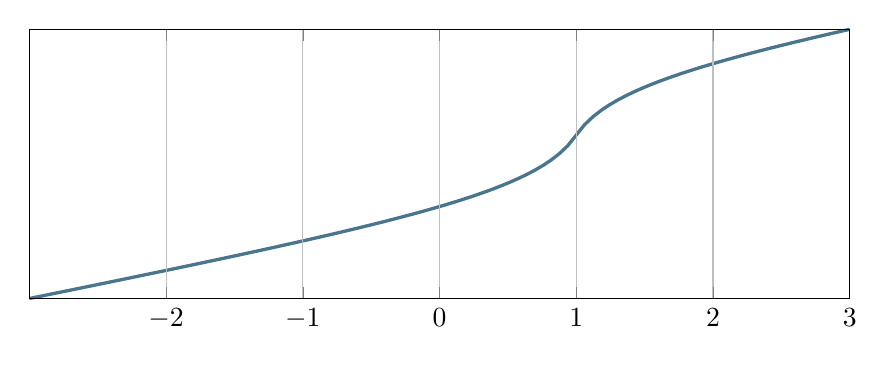
\begin{tikzpicture}
    \begin{axis}[
        no markers, domain=-3:3, samples=100,
        every axis y label/.style={at=(current axis.above origin),anchor=south},
        every axis x label/.style={at=(current axis.right of origin),anchor=west},
        height=5cm, width=12cm,
        xtick={-2,-1,0,1,2,3}, ytick=\empty,
        enlargelimits=false, clip=false, axis on top,
        grid = major
        ]
        \addplot [very thick,cyan!50!black] {
            sign(x - 1) * (ln(exp(abs(x - 1)) + exp(-2) - 1) + 2)
            };
    \end{axis}
    \end{tikzpicture}
\end{document}